\section{Ontological model of domestic environment}
It is expected that mobile robots undertake various tasks not only in industrial fields such as manufacturing plants and construction sites, but also in the environment we live in.

\subsection{Tbox}
In this project a generic home domain model has been taken into account. 

\begin{figure}[H]
\centering
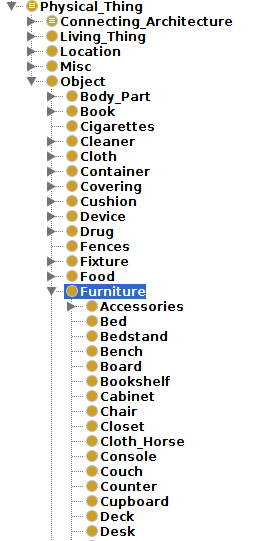
\includegraphics[width=0.3\textwidth]{imgs/ontology.png}
\label{fig:ontologyThings}
\caption{Taxonomy of classes in Prot\'eg\'e}
\end{figure}

The furniture class describes several objects of a domestic environment a robot can interact with.

\begin{figure}[H]
\centering
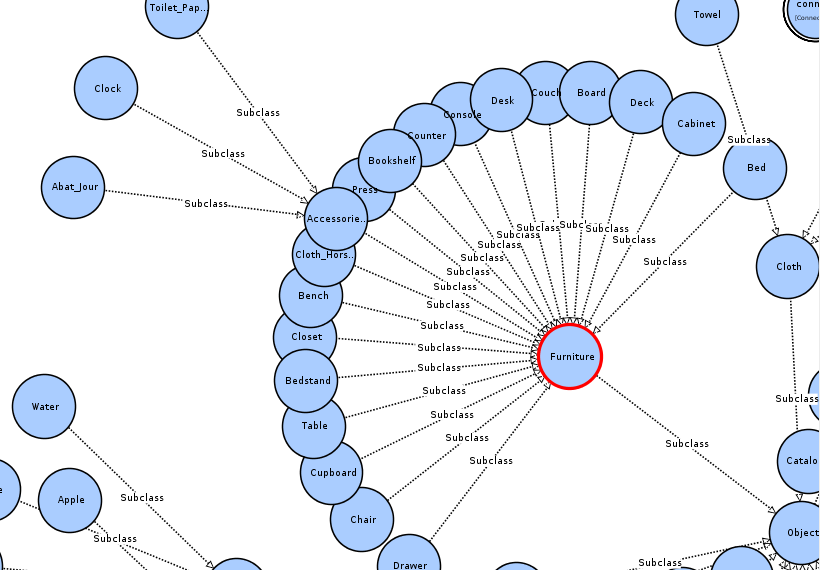
\includegraphics[width=0.8\textwidth]{imgs/ontology1.png}
\label{fig:furniture}
\caption{Furniture subclasses graph}
\end{figure}

As an example, consider the Coordinates class below.

\begin{lstlisting}[language=Java,basicstyle=\fontsize{9}{9}\selectfont\ttfamily]
<owl:Class rdf:about="sm#Coordinates">
    <rdfs:subClassOf rdf:resource="sm#Position"/>
    <rdfs:subClassOf>
       <owl:Restriction>
           <owl:onProperty rdf:resource="sm#float_coordinates_z"/>
           <owl:someValuesFrom 
           rdf:resource="http://www.w3.org/2001/XMLSchema#float"/>
           </owl:Restriction>
     </rdfs:subClassOf>
     <rdfs:subClassOf>
        <owl:Restriction>
           <owl:onProperty rdf:resource="sm#float_coordinates_x"/>
           <owl:qualifiedCardinality rdf:datatype="http://www.w3.org/2001/
           XMLSchema#nonNegativeInteger">
           </owl:qualifiedCardinality>
           <owl:onDataRange rdf:resource="http://www.w3.org/2001/XMLSchema#float"/>
           </owl:Restriction>
     </rdfs:subClassOf>
     <rdfs:subClassOf>
        <owl:Restriction>
           <owl:onProperty rdf:resource="sm#float_coordinates_y"/>
           <owl:qualifiedCardinality rdf:datatype="http://www.w3.org/2001/
           XMLSchema#nonNegativeInteger">
			</owl:qualifiedCardinality>
           <owl:onDataRange rdf:resource="http://www.w3.org/2001/XMLSchema#float"/>
       </owl:Restriction>
   </rdfs:subClassOf>
</owl:Class>   
\end{lstlisting}

The class Coordinates is a subclass of the class Position and of three anonymous classes. A property restriction describes an anonymous class, namely a class of all individuals that satisfy the restriction. \\\
The first restriction is a Value contraint that links (using owl:onProperty) the Property float\_coordinates\_z  to a class of all individuals for which at least one value of the property concerned is an instance of a data value in the data range.\\
The second and third restrictions are Cardinality contraints linked to the Property float\_coordinates\_x and float\_coordinates\_y.

\subsection*{Properties}
OWL distinguishes between two main categories of properties that an ontology builder may want to define:

\begin{itemize}
	\item Object properties link individuals to individuals.
	\item Datatype properties link individuals to data values.
\end{itemize}

An object property is defined as an instance of the built-in OWL class owl:ObjectProperty. A datatype property is defined as an instance of the built-in OWL class owl:DatatypeProperty. Both owl:ObjectProperty and owl:DatatypeProperty are subclasses of the RDF class rdf:Property.\\

\subsubsection*{Datatype Properties}
The datatypes involved are shown in the Figure ~\ref{fig:datatypes} and ~\ref{fig:datatypesProtege}

\begin{figure}[H]
\centering
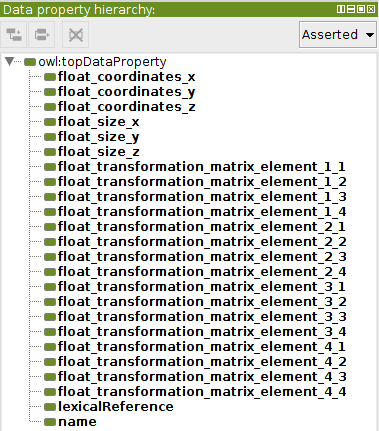
\includegraphics[width=0.6\textwidth]{imgs/datatypeProtege.png}
\label{fig:datatypesProtege}
\caption{Datatypes Visualization in Prot\'eg\'e}
\end{figure}

\begin{figure}[H]
\centering
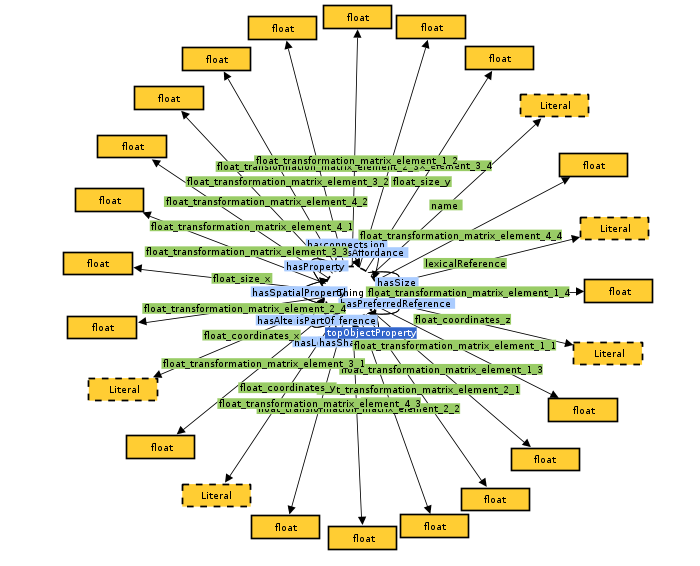
\includegraphics[width=0.6\textwidth]{imgs/Datatype.png}
\label{fig:datatypes}
\caption{Datatypes}
\end{figure}

\subsubsection*{Object Properties}

The following Figure \ref{fig:propClassTree} shows the class tree diagram of the ObjectProperties involved in the project.
\begin{figure}[H]
\centering
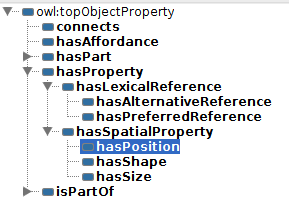
\includegraphics[width=0.6\textwidth]{imgs/propClassTree.png}
\label{fig:propClassTree}
\caption{Object Properties Class Tree}
\end{figure}

As an example, consider the following set of owl statements about the ObjectProperty hasPosition. This property is of the type IrreflexiveProperty and is a subProperty of SpacialProperty.

\begin{lstlisting}[language=Java,basicstyle=\fontsize{9}{9}\selectfont\ttfamily]
<owl:ObjectProperty rdf:about="sm#hasPosition">
    <rdfs:subPropertyOf rdf:resource="sm#hasSpatialProperty"/>
    <rdf:type rdf:resource="http://www.w3.org/2002/07/owl#IrreflexiveProperty"/>
</owl:ObjectProperty>
\end{lstlisting}    


\subsection{Abox}
\label{subsec:abox}
The collection of individual are stored in a separate file called semantic\_mapping, the Abox. The demo supports operations on four classes of instances since the 3D environment requires 3D models of the object to be represented. This constrain could be relaxed by adding an exhaustive collection of 3D models and by associating them to the corresponding classes.\\

\subsubsection*{An instance of the class Chair}
Individuals are defined with individual axioms called ``facts''. These facts are statements indicating class membership of individuals and property values of individuals. As an example, consider the following set of statements about an instance of the class Chair:

\begin{lstlisting}    [language=Java,basicstyle=\fontsize{9}{9}\selectfont\ttfamily]
<NamedIndividual rdf:about="sm#chair1">
        <rdf:type rdf:resource="&semantic_mapping_domain_model;Chair"/>
        <semantic_mapping_domain_model:hasPosition 
        rdf:resource="sm#chair1_coordinates"/>
        <semantic_mapping_domain_model:hasSize 
        rdf:resource="sm#chair1_size"/>
        <semantic_mapping_domain_model:hasAlternativeReference rdf:resource="sm#chair_alternative_reference_1"/>
        <semantic_mapping_domain_model:hasAlternativeReference   rdf:resource="sm#chair_alternative_reference_2"/>
        <semantic_mapping_domain_model:hasAlternativeReference  rdf:resource="sm#chair_alternative_reference_3"/>
        <semantic_mapping_domain_model:hasPreferredReference rdf:resource="sm#chair_preferred_reference"/>
    </NamedIndividual>
\end{lstlisting}

This example includes a number of facts about the individual chair1, an instance of the class Chair. The chair has three alternative references and one preferred lexical reference. These properties link a chair to a typed literal with the XML Schema datatype date. The XML schema document on datatypes contains the relevant information about syntax and semantics of this datatype. The property hasPosition and hasSize link the chair to instances of the type Coordinates and Dimensions.

The following figure shows the same information on Prot\'eg\'e:

\begin{figure}[H]
\centering
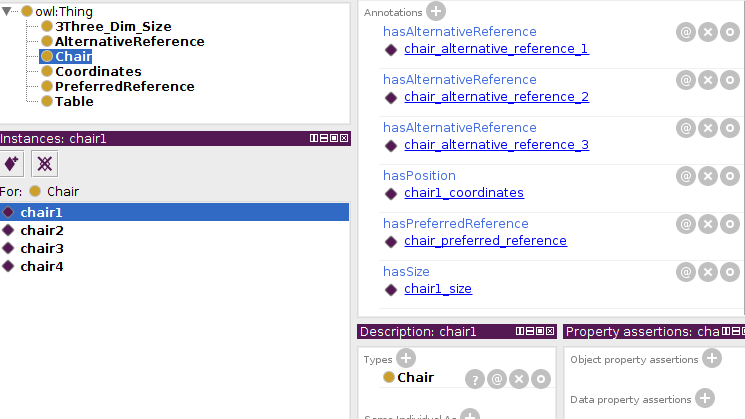
\includegraphics[width=0.6\textwidth]{imgs/chair1.png}
\label{fig:datatypes}
\caption{Chair1}
\end{figure}

\textbf{Properties}

The following example shows AlternativeReference instance property.
\begin{lstlisting}   [language=Java,basicstyle=\fontsize{9}{9}\selectfont\ttfamily] 
<NamedIndividual rdf:about="sm#chair_alternative_reference_1">
 <rdf:type rdf:resource="&semantic_mapping_domain_model;AlternativeReference"/>  <semantic_mapping_domain_model:lexicalReference rdf:datatype="&xsd;string">chair
 </semantic_mapping_domain_model:lexicalReference>
</NamedIndividual>
\end{lstlisting}


\begin{figure}[H]
\centering
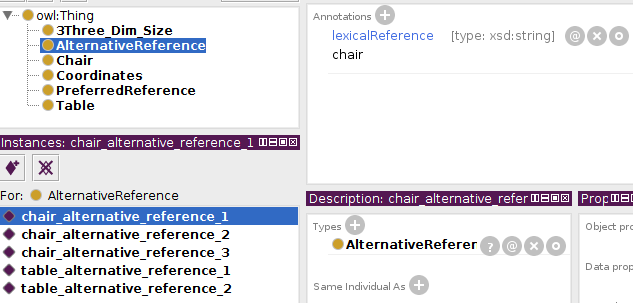
\includegraphics[width=0.6\textwidth]{imgs/refChair1.png}
\label{fig:datatypes}
\caption{Alternative Reference 1}
\end{figure}

The following example shows the instance of the 3Three\_Dim\_Size property associated to the individual chair1
\begin{lstlisting} [language=Java,basicstyle=\fontsize{9}{9}\selectfont\ttfamily]   
<NamedIndividual rdf:about="sm#chair1_coordinates">
        <rdf:type rdf:resource="&semantic_mapping_domain_model;Coordinates"/>
        <semantic_mapping_domain_model:float_coordinates_z 
        rdf:datatype="&xsd;float">0.0
        </semantic_mapping_domain_model:float_coordinates_z>
        <semantic_mapping_domain_model:float_coordinates_y 
        rdf:datatype="&xsd;float">0.0
        </semantic_mapping_domain_model:float_coordinates_y>
        <semantic_mapping_domain_model:float_coordinates_x 
        rdf:datatype="&xsd;float">1.0
        </semantic_mapping_domain_model:float_coordinates_x>
</NamedIndividual>
\end{lstlisting}



\begin{figure}[H]
\centering
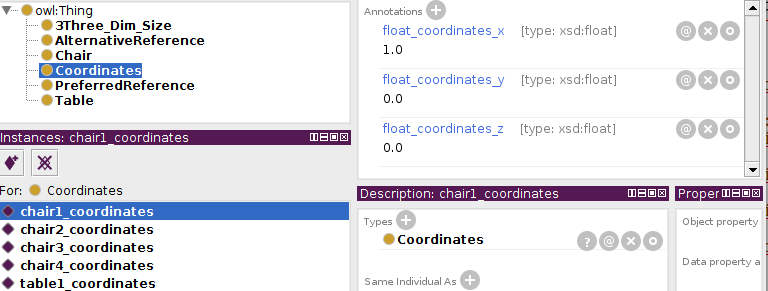
\includegraphics[width=0.6\textwidth]{imgs/coordchair1.png}
\label{fig:datatypes}
\caption{Coordinates chair 1}
\end{figure}
